\documentclass[tikz,border=10pt]{standalone}
\usepackage{amsmath,amssymb}
\usepackage{tikz}
\usetikzlibrary{arrows.meta,calc,positioning}

\definecolor{navy}{HTML}{1B365D}
\definecolor{steelblue}{HTML}{2471A3}
\definecolor{softblue}{HTML}{D4E6F1}
\definecolor{teal}{HTML}{0E6251}
\definecolor{amber}{HTML}{D35400}
\definecolor{crimson}{HTML}{C0392B}
\definecolor{slate}{HTML}{566573}

\begin{document}
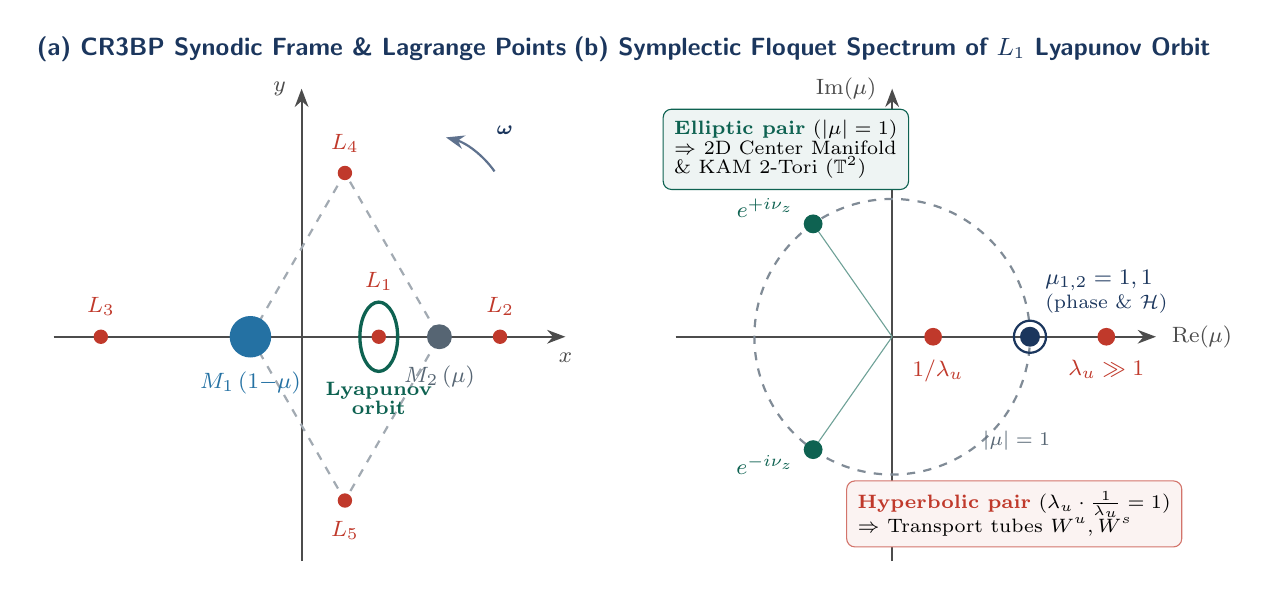
\begin{tikzpicture}[
    >=Stealth,
    font=\sffamily\small,
]

% ========================
% LEFT PANEL: CR3BP Synodic Frame & 5 Lagrange Points
% ========================
\begin{scope}[shift={(0,0)}]
    \node[font=\sffamily\bfseries\small, navy] at (0.0, 3.65)
        {(a) CR3BP Synodic Frame \& Lagrange Points};

    % Axes
    \draw[->, thick, black!70] (-3.15, 0) -- (3.35, 0) node[below=2pt, font=\footnotesize] {$x$};
    \draw[->, thick, black!70] (0, -2.85) -- (0, 3.15) node[left=2pt, font=\footnotesize] {$y$};

    % Primaries (exaggerated mu for clarity: M1 at (-0.65,0), M2 at (1.75,0), dist = 2.4)
    \coordinate (M1) at (-0.65, 0);
    \coordinate (M2) at (1.75, 0);
    \coordinate (L1) at (0.98, 0);
    \coordinate (L2) at (2.52, 0);
    \coordinate (L3) at (-2.55, 0);
    % Equilateral triangles of side 2.4: mid x = 0.55, height = 2.4*sqrt(3)/2 = 2.078
    \coordinate (L4) at (0.55, 2.08);
    \coordinate (L5) at (0.55, -2.08);

    % Equilateral triangle dashed lines
    \draw[dashed, slate!55, thick] (M1) -- (L4) -- (M2) -- (L5) -- (M1);

    % Small planar Lyapunov orbit around L1
    \draw[teal, very thick] (L1) ellipse (0.24 and 0.44);
    \node[teal, font=\scriptsize\bfseries, align=center] at (0.98, -0.78)
        {Lyapunov\\[-1pt]orbit};

    % Primaries
    \fill[steelblue] (M1) circle (7.5pt);
    \node[steelblue, font=\footnotesize\bfseries, below=9pt] at (M1) {$M_1\,(1{-}\mu)$};

    \fill[slate] (M2) circle (4.5pt);
    \node[slate, font=\footnotesize\bfseries, below=7pt] at (M2) {$M_2\,(\mu)$};

    % Lagrange points
    \fill[crimson] (L1) circle (2.6pt);
    \node[crimson, font=\footnotesize\bfseries, above=13pt] at (L1) {$L_1$};
    \fill[crimson] (L2) circle (2.6pt);
    \node[crimson, font=\footnotesize\bfseries, above=4pt] at (L2) {$L_2$};
    \fill[crimson] (L3) circle (2.6pt);
    \node[crimson, font=\footnotesize\bfseries, above=4pt] at (L3) {$L_3$};
    \fill[crimson] (L4) circle (2.6pt);
    \node[crimson, font=\footnotesize\bfseries, above=4pt] at (L4) {$L_4$};
    \fill[crimson] (L5) circle (2.6pt);
    \node[crimson, font=\footnotesize\bfseries, below=4pt] at (L5) {$L_5$};

    % Rotation indicator
    \draw[->, thick, navy!70] (2.45, 2.10) arc[start angle=35, end angle=75, radius=1.1];
    \node[navy, font=\scriptsize] at (2.58, 2.62) {$\boldsymbol{\omega}$};
\end{scope}

% ========================
% RIGHT PANEL: Symplectic Floquet Multipliers of 6D Planar L1 Lyapunov Orbit
% ========================
\begin{scope}[shift={(7.5, 0)}]
    \node[font=\sffamily\bfseries\small, navy] at (0.0, 3.65)
        {(b) Symplectic Floquet Spectrum of $L_1$ Lyapunov Orbit};

    % Complex plane axes
    \draw[->, thick, black!70] (-2.75, 0) -- (3.35, 0) node[right=2pt, font=\footnotesize] {$\operatorname{Re}(\mu)$};
    \draw[->, thick, black!70] (0, -2.85) -- (0, 3.15) node[left=2pt, font=\footnotesize] {$\operatorname{Im}(\mu)$};

    % Unit circle S^1
    \draw[thick, dashed, slate!75] (0,0) circle (1.75);
    \node[slate, font=\scriptsize] at (1.58, -1.32) {$|\mu| = 1$};

    % Trivial double multiplier mu = 1, 1
    \fill[navy] (1.75, 0) circle (3.6pt);
    \draw[navy, thick] (1.75, 0) circle (5.8pt);
    \node[navy, font=\footnotesize\bfseries, align=left, above right=5pt and 2pt] at (1.75, 0)
        {$\mu_{1,2} = 1, 1$\\[-1pt]\normalfont\scriptsize (phase \& $\mathcal{H}$)};

    % Hyperbolic pair: lambda_u > 1 and 1/lambda_u < 1
    \fill[crimson] (2.72, 0) circle (3.2pt);
    \node[crimson, font=\footnotesize\bfseries, below=5pt] at (2.72, 0) {$\lambda_u \gg 1$};
    \fill[crimson] (0.52, 0) circle (3.2pt);
    \node[crimson, font=\footnotesize\bfseries, below=5pt] at (0.58, 0) {$1/\lambda_u$};

    % Elliptic pair on unit circle: e^{\pm i nu_z}
    \coordinate (ep) at (125:1.75);
    \coordinate (em) at (-125:1.75);
    \draw[thin, teal!60] (0,0) -- (ep) (0,0) -- (em);
    \fill[teal] (ep) circle (3.4pt);
    \fill[teal] (em) circle (3.4pt);
    \node[teal, font=\footnotesize\bfseries, anchor=east] at ($(ep) + (-0.12, 0.20)$) {$e^{+i\nu_z}$};
    \node[teal, font=\footnotesize\bfseries, anchor=east] at ($(em) + (-0.12, -0.20)$) {$e^{-i\nu_z}$};

    % Annotation for elliptic pair -> KAM 2-tori
    \node[draw=teal, fill=teal!7, rounded corners=3pt, font=\scriptsize, align=left, inner sep=4pt]
        at (-1.35, 2.38) {\textbf{\color{teal}Elliptic pair} ($|\mu|=1$)\\[-1pt]$\Rightarrow$ 2D Center Manifold\\[-1pt]\& KAM 2-Tori ($\mathbb{T}^2$)};

    % Annotation for hyperbolic pair -> invariant manifold tubes
    \node[draw=crimson!70, fill=crimson!6, rounded corners=3pt, font=\scriptsize, align=left, inner sep=4pt]
        at (1.55, -2.25) {\textbf{\color{crimson}Hyperbolic pair} ($\lambda_u \cdot \frac{1}{\lambda_u} = 1$)\\[-1pt]$\Rightarrow$ Transport tubes $W^u, W^s$};
\end{scope}

\end{tikzpicture}
\end{document}
